\documentclass{beamer}

\usepackage{beamerthemesplit}% // Activate for custom appearance

\title{$\chi$pods and Mixing Efficiency}
\author{Andy Pickering}
\date{\today}

\graphicspath{
{/Users/Andy/Cruises_Research/Analysis/Andy_Pickering/tiwe_patch_gamma/figures/}
{/Users/Andy/Cruises_Research/Analysis/Andy_Pickering/eq14_patch_gamma/figures/}
}

\begin{document}

\frame{\titlepage}

\section[Outline]{}
\frame{\tableofcontents}


%~~~~~~~~~~~~~~~~~~~~~~~~~~~~~~
\section{Introduction}
%~~~~~~~~~~~~~~~~~~~~~~~~~~~~~~


%~~~~~~~~~
\begin{frame}
 \frametitle{The CTD-$\chi$pod}

   \begin{itemize}
  \item Measures temperature gradient w/ FP07 thermistor
  \item Easily deployed on traditional CTD, Tz not as sensitive to package vibration
  \item Goal is to be able to estimate $\chi$ and $\epsilon$ w/o full microstructure
  \end{itemize}

\end{frame}


%~~~~~~~~~
\begin{frame}
 \frametitle{$\chi$pod Method}

In small windows:
   \begin{itemize}
  \item Convert dT/dt to dT/dz using fallspeed
  \item  Compute spectra of dT/dz
  \item Iterative method to estimate $\chi$,$\epsilon$
  \item Assumes $K_T=K_{\rho}$
  \item Assumes mixing efficency (coefficient) $\gamma=0.2$
  \end{itemize}

\end{frame}



%~~~~~~~~~
\begin{frame}
 \frametitle{CTD-$\chi$pod Validation}

   \begin{itemize}
  \item To validate, compare w/ Chamelon microstructure profiles (1m avg).
  \item Apply $\chi$pod method to Chameleon thermistor data only (no shear probes)
  \item Compare to Chameleon estimates using shear probes.
  \end{itemize}

Results:
   \begin{itemize}
  \item $\chi$ compares well
  \item $\epsilon$ biased low by about 10X
    \end{itemize}

\end{frame}




%~~~~~~~~~
\begin{frame}
 \frametitle{Why is $\epsilon$ Biased so Low?}

Turns out using the 1m avg Chameleon data, $\gamma \approx 0.02$, not 0.2  .
\begin{equation}
\gamma_{\chi\epsilon}=\frac{N^2 \chi}{2\epsilon T_{z}^{2}} 
\end{equation}

Apparently Sasha found something similar for EQ08 and other Chameleond datasets.

\end{frame}



%~~~~~~~~~
\begin{frame}
 \frametitle{What if We Compute $\gamma$ over patches?}
\begin{itemize}
\item But everyone says $\gamma=0.2$...
\item Maybe we have to compute it over patches. If there's no mixing, does $\gamma$ even make sense?
\end{itemize}

\end{frame}





%~~~~~~~~~
\begin{frame}
 \frametitle{Patches}
\begin{itemize}
\item Turns out computing $\gamma$ over patches not so simple...
\item Lots of options for how to identify patches, calculate $T_z$ and $N^2$ etc.
\item Lots of salinity spikes, need to use temperature.
\item Use 60-200m only (don't include diurnal cycle turbulence etc.)
\end{itemize}

\end{frame}



%~~~~~~~~~
\begin{frame}
 \frametitle{Salinity spikes}
\begin{itemize}
\item Salinity looks noisy, lots of spikes.
\item Not a constant T-S relationship 
\item use $R^2$ to quanity `tight' T-S relationships in patches?
\end{itemize}


\begin{figure}[htbp]
\begin{center}
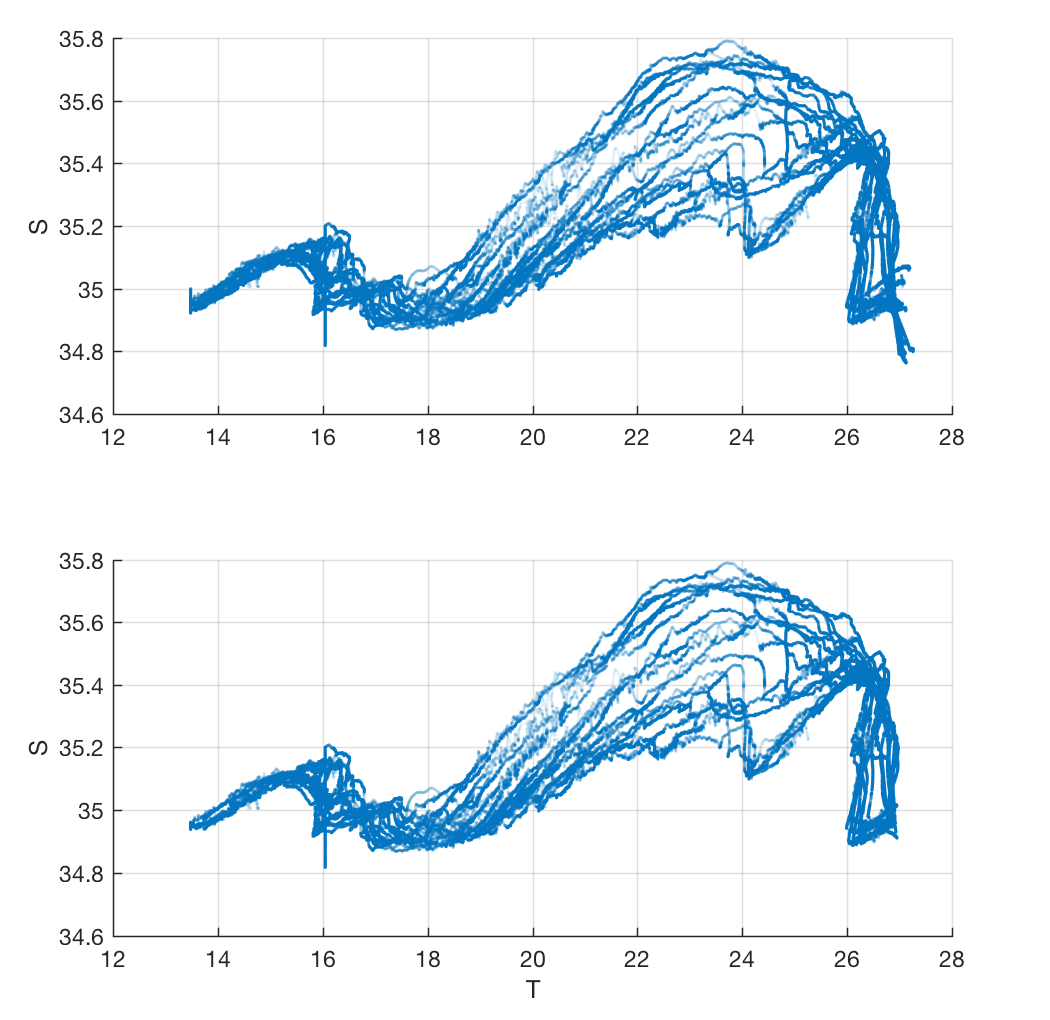
\includegraphics[scale=0.25]{tiwe_T_S_scatter.png}
\caption{default}
\label{default}
\end{center}
\end{figure}


\end{frame}




%~~~~~~~~~
\begin{frame}
 \frametitle{dT/dz and N2}
 
$T_z$:
\begin{itemize}
\item $T_z$ `'line' : Fit a straight line to sorted temperature within patch.
\item $T_z$ `bulk' : Method from Smyth et al 2001. More robust when there are multiple layers within patch?
\end{itemize}

$N^2$:
\begin{itemize}
\item $N^2$ `'line' : Fit a straight line to sorted density within patch.
\item $N^2$ `'fit' : Fit a straight line to density computed from T-S fit in patch.
\item $N^2$ `bulk' : Use `bulk' $T_z$, and ratio between density and temperature.
\end{itemize}


\end{frame}




%~~~~~~~~~
\begin{frame}
 \frametitle{$\gamma$}

This gives us 4 estimates of $\gamma$: 
\begin{itemize}
\item $\gamma$ bin : Binned $T_z$,$N^2$ interopolated to patch locations.
\item $\gamma$ `'line' : `line' $T_z$,$N^2$
\item $\gamma$ `bulk' : `bulk' $T_z$,$N^2$
\item $\gamma$ `linefit' : `line' $T_z$,, `'line-fit' $N^2$
\end{itemize}

\end{frame}



%~~~~~~~~~~~~~~~~~~~~~~~~~~~~~~~~~~~~~~~~~
\section{TIWE}


%~~~~~~~~~
\begin{frame}
 \frametitle{Overview}

\begin{columns}
\column{0.5\textwidth}
\begin{itemize}
\item 
\end{itemize}

\column{0.5\textwidth}
\begin{figure}[htbp]
\begin{center}
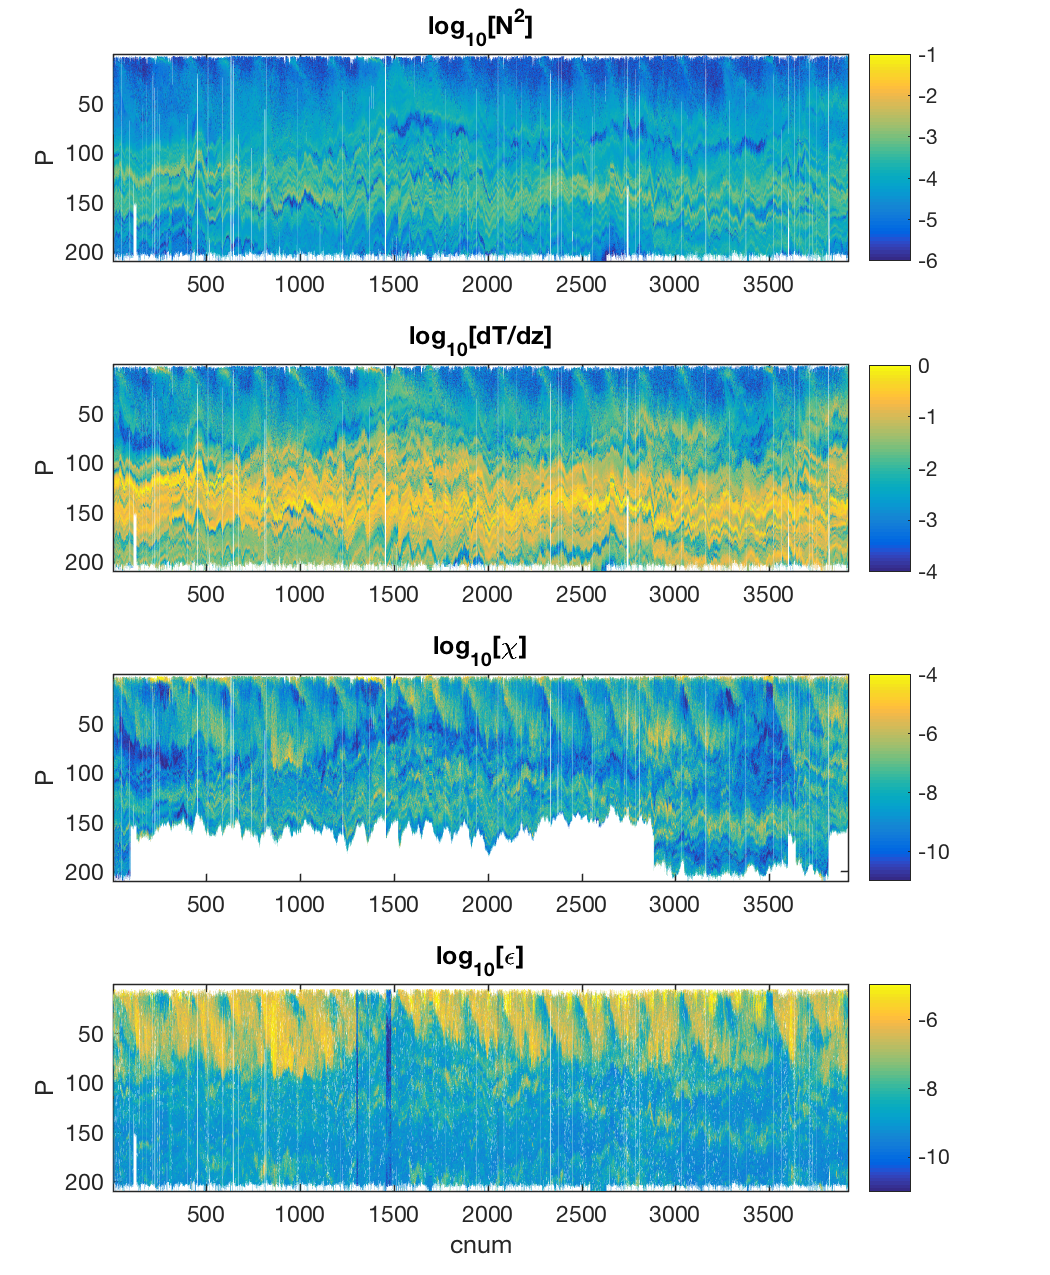
\includegraphics[scale=0.3]{tiwe_avgCombine_N2_dtdz_chi_eps.png}
\caption{}
\label{default}
\end{center}
\end{figure}

\end{columns}


\end{frame}


%~~~~~~~~~
\begin{frame}
 \frametitle{TIWE binned}

\begin{columns}
\column{0.5\textwidth}
\begin{itemize}
\item Looked at TIWE 1st because there were some previous patch analayis and gamma estimates (Bill,Jim).
\item Binned gamma has median of ...
\end{itemize}

\column{0.5\textwidth}
\begin{figure}[htbp]
\begin{center}
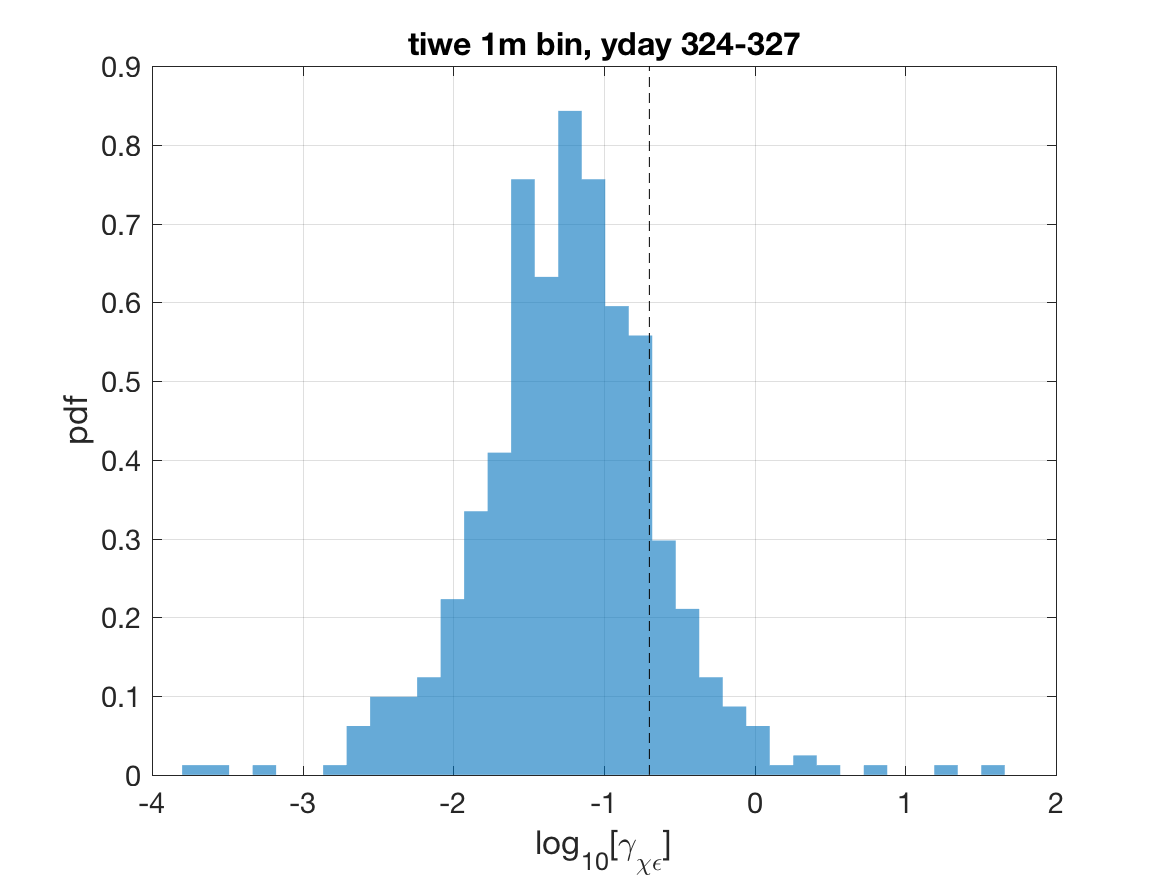
\includegraphics[scale=0.3]{tiwe_avgCombine_gamma_yday_324_327.png}
\caption{$\gamma$ estimated from 1m binned TIWE profiles.}
\label{default}
\end{center}
\end{figure}

\end{columns}


\end{frame}


%~~~~~~~~~
\begin{frame}
 \frametitle{TIWE patch}

\begin{columns}
\column{0.5\textwidth}
\begin{itemize}
\item Patch estimates of $\gamma$ are all equal or greater than 0.2
\item 
\end{itemize}

\column{0.5\textwidth}
\begin{figure}[htbp]
\begin{center}
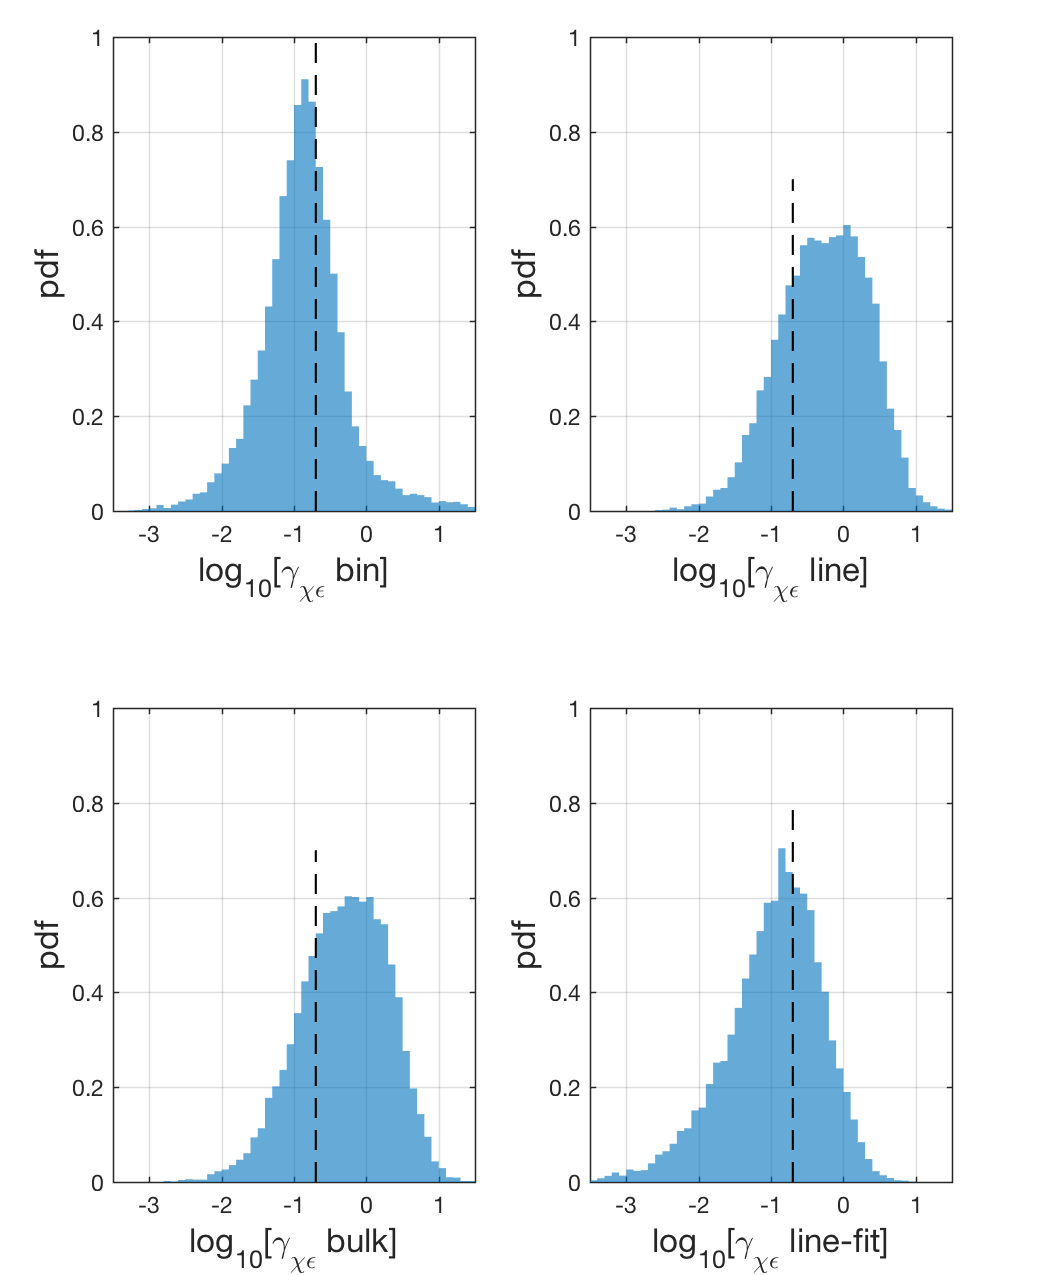
\includegraphics[scale=0.25]{tiwe_minOT_40_usetemp_1_gammas_hist2X2_yday_324_327.png}
\caption{default}
\label{default}
\end{center}
\end{figure}

\end{columns}


\end{frame}





%~~~~~~~~~
\begin{frame}
 \frametitle{Results table}


\begin{table}[htdp]
\caption{Statistics for patches using various parameters. $\gamma$ values are medians for each distribution. Only patches between 60-200m and on yday 324-327 are considered for all.}
\begin{center}
\begin{tabular}{|c|c|c|c|c|c|c|c|}
\hline
minOT & usetemp & minR2 & $\gamma bin$ & $\gamma line$ & $\gamma fit$ & $\gamma bulk$ & Npatches \\
\hline
0.4 & 1 & 0 & 0.13 & 0.57 & 0.11 & 0.53 & 16329 \\
\hline
0.4 & 1 & 0.5 & 0.14 & 0.22 & 0.12 & 0.21 & 3761 \\
\hline
0.75 & 1 & 0 & 0.15 & 0.62 & 0.14 & 0.59 & 9175 \\
\hline
0.75 & 1 & 0.5 & 0.15 & 0.25 & 0.16 & 0.26 & 2358 \\
\hline
1 & 1 & 0 & 0.16 & 0.71 & 0.15 & 0.68 & 6893 \\
\hline
1 & 1 & 0.5 & 0.16 & 0.29 & 0.17 & 0.29 & 1779 \\
\hline
\hline
\hline
\end{tabular}
\end{center}
\label{tab}
\end{table}%


\end{frame}




%~~~~~~~~~~~~~~~~~~~~~~~~~~~~~~~~~~~~~~~~~
\section{EQ14}

%~~~~~~~~~
\begin{frame}
 \frametitle{EQ14 1}


\end{frame}


%~~~~~~~~~
\begin{frame}
 \frametitle{EQ14 2}


\begin{columns}
\column{0.5\textwidth}
\begin{itemize}
\item Patch estimates of $\gamma$ are ..
\item 
\end{itemize}

\column{0.5\textwidth}
\begin{figure}[htbp]
\begin{center}
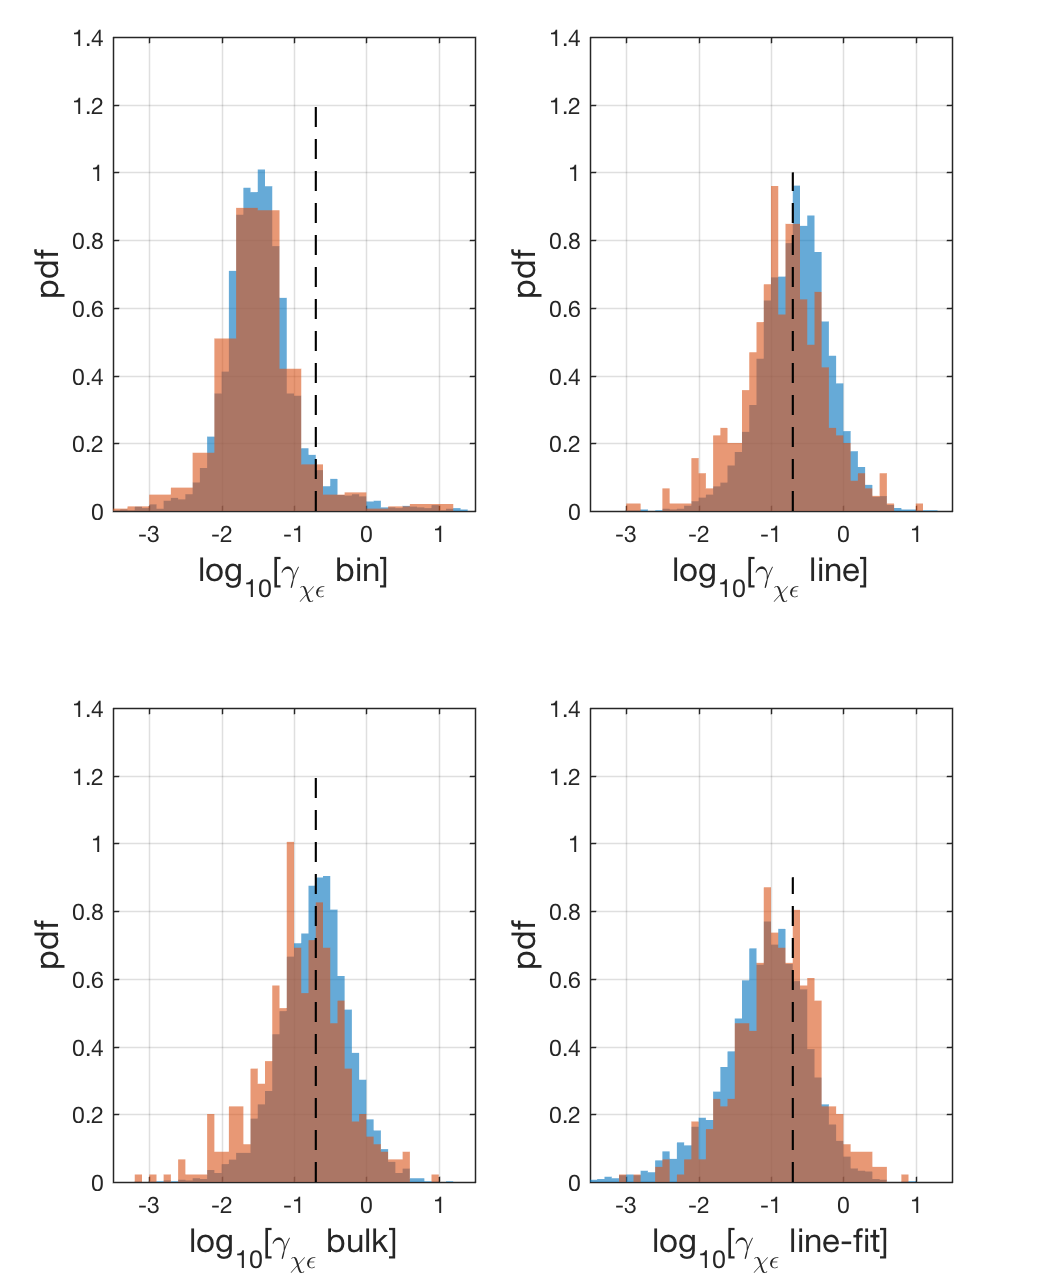
\includegraphics[scale=0.25]{eq14_minOT_40_usetemp_1_gammas_hist2X2_depth_80_200m.png}
\caption{default}
\label{default}
\end{center}
\end{figure}

\end{columns}



\end{frame}



%~~~~~~~~~
\begin{frame}
 \frametitle{ EQ14 3}

\begin{table}[htdp]
\caption{Statistics for patches using various parameters. $\gamma$ values are medians for each distribution. Only patches between 60-200m are considered.}
\begin{center}
\begin{tabular}{|c|c|c|c|c|c|c|c|}
\hline
minOT & usetemp & minR2 & $\gamma bin$ & $\gamma line$ & $\gamma fit$ & $\gamma bulk$ & Npatches \\
\hline
0.4 & 1 & 0 & 0.03 & 0.15 & 0.02 & 0.13 & 9326 \\
\hline
0.4 & 1 & 0.5 & 0.03 & 0.09 & 0.02 & 0.08 & 1301 \\
\hline
0.75 & 1 & 0 & 0.05 & 0.13 & 0.02 & 0.12 & 4075 \\
\hline
0.75 & 1 & 0.5 & 0.05 & 0.08 & 0.03 & 0.08 & 520 \\
\hline
1 & 1 & 0 & 0.06 & 0.12 & 0.02 & 0.12 & 2829 \\
\hline
1 & 1 & 0.5 & 0.05 & 0.08 & 0.04 & 0.08 & 387 \\
\hline
\hline
\hline
\end{tabular}
\end{center}
\label{tab}
\end{table}%


\end{frame}


%~~~~~~~~~~~~~~~~~~~~~~~~~~~~~~~~
\section{Applying $\chi$pod method to patches}

\begin{frame}
 \frametitle{ }
 
 \begin{figure}[htbp]
\begin{center}
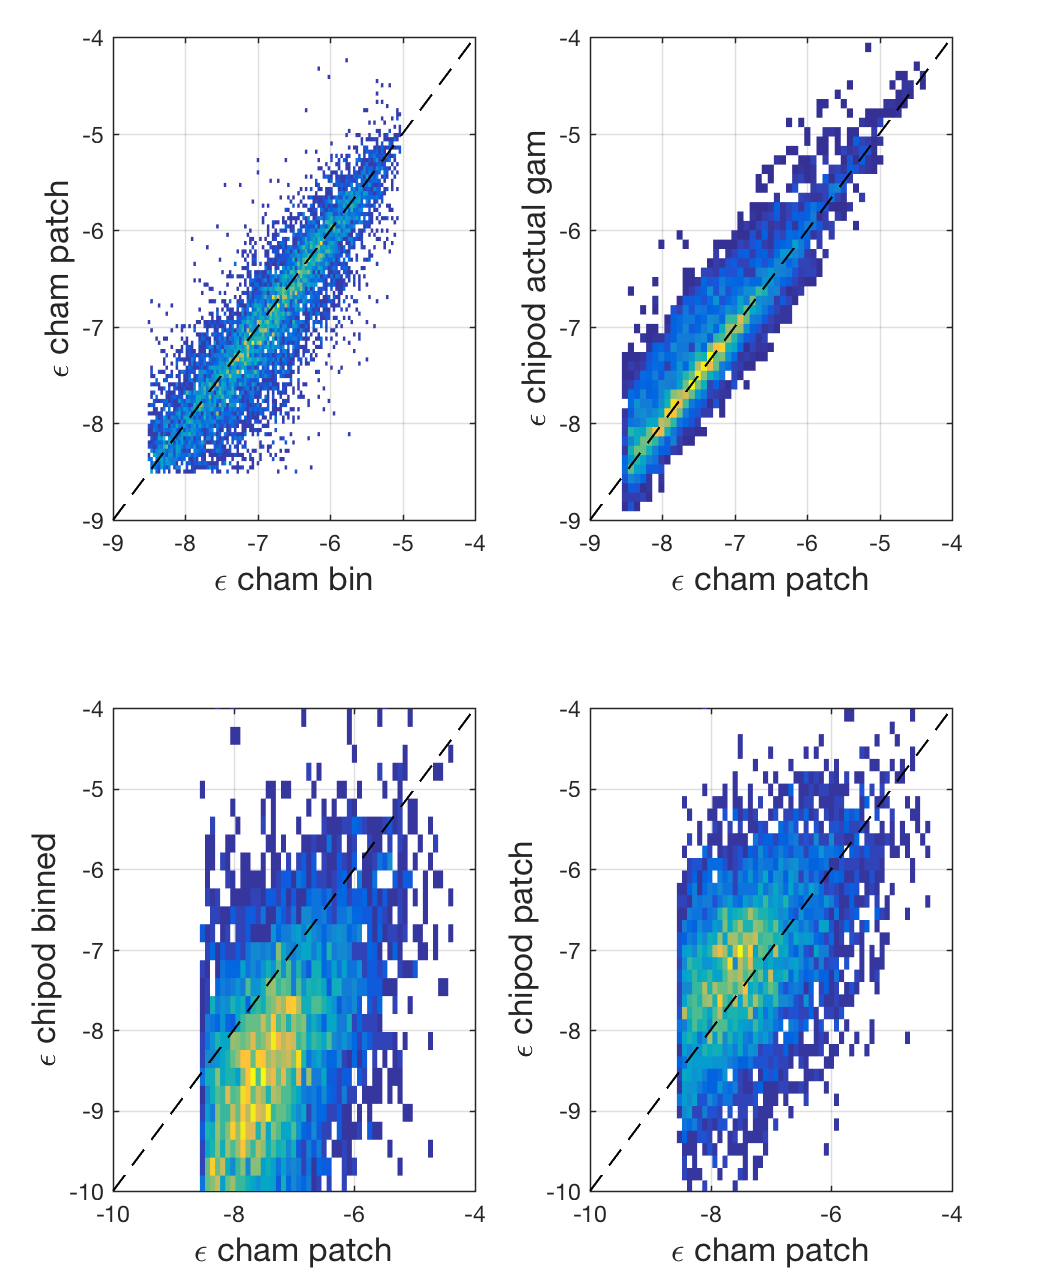
\includegraphics[scale=0.3]{ChiPatchEpsCompare_N2dTdz_line_minOT40_usetemp_1.png}
\caption{default}
\label{default}
\end{center}
\end{figure}


\end{frame}




%~~~~~~~~~~~~~~~~~~~~~~~~~~~~~~~~
\section{Summary}

\begin{frame}
 \frametitle{ Summary}

\begin{itemize}
\item 
\end{itemize}


\end{frame}



%~~~~~~~~~~~~~~~~~~~~~~~~~~~~~~
\end{document}
%~~~~~~~~~~~~~~~~~~~~~~~~~~~~~~